\newpage
\pagestyle{fancy}

\lhead{\textsc{Chapitre 5. Tests et validation expérimentale}}
\renewcommand{\headrulewidth}{0.5pt}
\renewcommand{\footrulewidth}{0.5pt}
\chapter{Tests et validation expérimentale}\setlength{\headheight}{27.06pt}
\label{ch5}
\minitoc

\newpage
\section{Introduction}
\label{sec:tests-introduction}

Le chapitre 1 a formulé une problématique et proposé xQoS comme réponse ; les chapitres 3 et 4 ont ensuite permis de concevoir et d'implémenter cette proposition. Restait une question qu'aucun de ces chapitres ne pouvait trancher : \textbf{le système construit tient-il, en pratique, les promesses formulées ?} Trois affirmations, en particulier, appellent une vérification empirique : qu'une intention exprimée en langage naturel est traduite fidèlement en objectifs mesurables, qu'une dégradation est anticipée avant d'être subie et que plusieurs fournisseurs indépendants parviennent à coopérer sans qu'aucun ne dispose d'une autorité centrale sur les autres.

Ce chapitre apporte des éléments de réponse à ces questions à partir de mesures réalisées sur l'infrastructure réelle du LAAS-CNRS. Il s'ouvre sur la présentation du protocole expérimental suivi (section~\ref{sec:protocole}), puis présente les résultats du niveau le plus local au niveau le plus global : la traduction d'intention (section~\ref{sec:resultats-intention}), la prise de décision au sein d'un seul fournisseur (section~\ref{sec:resultats-decision-locale}), puis la coordination entre fournisseurs (section~\ref{sec:resultats-federation}). Une synthèse clôt cette analyse en confrontant les résultats obtenus à la problématique initiale et en explicitant les limites de l'évaluation (section~\ref{sec:synthese-limites}).

Tous les résultats rapportés dans ce chapitre ne sont pas nécessairement favorables au système : certains mettent en évidence ses performances, tandis que d'autres documentent des limites qui subsistent à ce stade. Ces deux catégories sont présentées avec la même rigueur, car leur analyse conjointe permet d'évaluer dans quelle mesure xQoS répond effectivement à la problématique posée.

\newpage
\section{Protocole expérimental}
\label{sec:protocole}

Cette section décrit le protocole expérimental sur lequel reposent les résultats présentés dans la suite du chapitre. Elle présente d'abord le banc d'essai et les scénarios exécutés (section~\ref{sec:protocole-scenarios}), puis les métriques retenues et la méthode statistique utilisée pour analyser les résultats (section~\ref{sec:protocole-metriques}).

\subsection{Banc d'essai et scénarios}
\label{sec:protocole-scenarios}

L'ensemble des résultats présentés dans ce chapitre a été obtenu sur l'infrastructure réelle du LAAS-CNRS, et non en simulation. Celle-ci comprend cinq machines virtuelles OpenStack orchestrées par Kubernetes. L'une d'elles héberge le plan de contrôle et exécute les migrations ; elle ne constitue pas une cible de placement. Les quatre autres se répartissent à parts égales entre les deux fournisseurs : une machine de type \emph{edge} et une machine de type \emph{cloud} pour chacun.

Sur chaque machine \emph{edge} s'exécutent trois agents indépendants, chacun sur son propre port, avec sa propre position géographique et sa propre capacité déclarée — deux, trois et quatre cœurs respectivement. Chaque machine \emph{cloud} n'héberge qu'un seul agent, de capacité nettement supérieure. L'orchestrateur dispose ainsi de huit cibles de placement distinctes, quatre par fournisseur, réparties sur quatre machines. Chacune de ces cibles étant perçue par le système comme une machine autonome — elle expose ses propres métriques, sa propre capacité et sa propre position —, la suite du chapitre les désigne par commodité sous le terme de VM, conformément à l'usage des journaux et des outils d'analyse.

Cette organisation a une conséquence directe sur l'observabilité, dont la section~\ref{sec:protocole-metriques} tire les implications : les trois cibles \emph{edge} d'un même fournisseur s'exécutant sur une seule machine, elles partagent le même nœud Kubernetes. Une résolution effectuée via \texttt{kubectl} ne peut donc pas les distinguer.

Les migrations déclenchées par le système ne correspondent pas à de simples changements d'état logiques, mais à de véritables déplacements de pods, exécutés via \texttt{kubectl} sur cette infrastructure.

Le signal de latence qui pilote le cycle de décision n'est pas un aléa généré en amont : il provient d'un robot PiCar-X piloté depuis un Raspberry Pi, dont la position réelle sur un parcours fixe est convertie en une latence simulée vis-à-vis de chaque VM, à l'aide d'une fonction déterministe de la distance. La trajectoire est ainsi identique d'une exécution à l'autre ; seule la réponse de l'orchestrateur diffère. Cette propriété permet de comparer les différentes exécutions dans des conditions aussi similaires que possible.

Il convient de préciser d'emblée que le banc décrit ici est celui sur lequel a été menée la campagne dont les résultats occupent l'essentiel de ce chapitre. Dans cette configuration, la latence dépend de la seule position du véhicule, tandis que les charges CPU et mémoire évoluent indépendamment. Cette indépendance, voulue à l'origine, s'est révélée limitante pour l'évaluation du mécanisme de découverte d'objectifs secondaires : le banc n'offrait aucune dépendance à découvrir. Le simulateur a donc été modifié ultérieurement pour coupler la charge CPU à la latence, ce que détaille la section~\ref{sec:validation-mi}. Sauf mention explicite du contraire, toutes les mesures rapportées dans ce chapitre proviennent de la configuration non couplée décrite ci-dessus.

\textbf{Deux conditions expérimentales.} Afin d'isoler la contribution propre de la fédération, deux conditions expérimentales ont été comparées en ne faisant varier qu'un seul paramètre :

\begin{table}[H]
    \centering
    \caption{Conditions expérimentales comparées}
    \label{tab:conditions-experimentales}
    \begin{tabular}{lcc}
        \toprule
        \textbf{Paramètre} & \textbf{Condition fédérée} & \textbf{Condition d'ablation} \\
        \midrule
        \texttt{MULTI\_PROVIDER\_ENABLED} & \texttt{true} & \texttt{false} \\
        Orchestrateurs actifs & provider-1 et provider-2 & provider-1 seul \\
        Cibles de placement disponibles & 8 & 4 \\
        Trajectoire, seuil et code & identiques & identiques \\
        \bottomrule
    \end{tabular}
\end{table}

La présence ou l'absence de la fédération constitue la seule différence expérimentale entre les deux conditions : le parcours du véhicule, le seuil de conformité et la base de code sont identiques. L'objectif est ainsi d'attribuer les écarts observés entre les deux conditions au mécanisme de fédération, sous réserve des autres sources de variabilité expérimentale.

\textbf{Scénario d'évaluation de la traduction d'intention (UC5).} Indépendamment de la campagne fédérée/ablation, la capacité du système à traduire une intention exprimée en langage naturel a été évaluée sur douze phrases issues d'un document tiers fourni par l'encadrant, décrivant un scénario de diffusion vidéo en véhicule. Ces phrases n'ont pas été rédigées pour le système qu'elles évaluent, ce qui écarte tout biais de formulation favorable. Elles couvrent délibérément des cas que de simples règles de correspondance ne couvriraient pas : des besoins implicites, pour lesquels la métrique concernée n'est jamais nommée, une exigence d'arbitrage inverse, des formulations vagues, ainsi que deux demandes situées hors du domaine des métriques observables par le système.

\textbf{État initial et préchauffage.} Chaque exécution démarre d'un état vierge : la base de données du fournisseur est purgée automatiquement au lancement, de sorte qu'aucune donnée de la session précédente ne subsiste dans les fenêtres d'historique. Cette purge est nécessaire, un historique mêlant deux sessions produisant une discontinuité artificielle que les modèles de prédiction n'ont jamais rencontrée à l'entraînement. Elle présente en outre une vertu méthodologique : les huit exécutions partent d'un état identique, ce qui rend la variabilité observée entre elles interprétable.

Cette purge impose en contrepartie une période de préchauffage, dont la durée dépend de la fenêtre d'entrée propre à chaque modèle. Ces fenêtres ne sont pas fixées par l'orchestrateur mais déclarées par les modèles eux-mêmes et relevées à chaque démarrage : quarante-cinq points pour la latence et la mémoire, vingt-cinq pour le CPU, soit respectivement quatre minutes trente et deux minutes trente au rythme d'un cycle toutes les six secondes. En deçà de ce seuil, le module de prédiction se replie silencieusement sur un niveau dégradé.

Le protocole prévoyait une fenêtre autonome de trois minutes avant la mise en mouvement du véhicule. Cette durée couvre la fenêtre du modèle de CPU, mais reste inférieure à celle des modèles de latence et de mémoire. Les premières minutes de roulage de chaque exécution reposent donc, pour ces deux métriques, sur des prédictions issues du niveau de repli plutôt que du modèle nominal. Cet écart, identifié a posteriori lors du dépouillement, contribue à la proportion de prédictions non nominales rapportée en section~\ref{sec:qualite-prediction}. Il affecte les huit exécutions de manière identique et ne peut donc favoriser l'une des deux conditions comparées, mais il constitue un écart au protocole qu'il convient de signaler.

Enfin, il faut souligner que cette réplication mesure la variabilité du comportement de l'orchestrateur — décisions, cadence, prédictions — et non celle de l'environnement : la trajectoire du véhicule étant déterministe et identique d'une exécution à l'autre, l'entrée du système ne varie pas d'un essai au suivant.

\textbf{Ampleur de la campagne.} La comparaison entre les conditions fédérée et d'ablation repose sur quatre exécutions indépendantes par condition, soit huit exécutions au total. Les exécutions ont été alternées au cours de la journée plutôt que regroupées par condition, afin qu'une éventuelle dérive de l'infrastructure au cours de la journée puisse affecter les deux conditions de manière comparable. Chaque exécution dure environ 55 minutes, dont un peu plus de 40 minutes de roulage effectif. Le choix de quatre exécutions par condition est justifié par la méthode statistique présentée dans la section~\ref{sec:protocole-metriques}, qui précise les conditions permettant d'évaluer la significativité des différences observées.

\subsection{Métriques et méthode statistique}
\label{sec:protocole-metriques}

\textbf{Taux de violation.} Il s'agit de l'indicateur central de ce chapitre : il correspond à la proportion du temps pendant laquelle le seuil de conformité en vigueur, fixé à une latence inférieure à 28~ms en mode autonome, n'est pas respecté par la VM qui héberge effectivement le service à cet instant. Il est calculé en croisant la trajectoire réelle du véhicule, dont la latence vis-à-vis de chaque VM est déterminée de manière déterministe, avec la VM effectivement active à chaque instant.

Ce dernier point mérite une précision méthodologique. Deux colonnes distinctes désignent la VM hôte dans les exports du système : l'une reflète l'état interne de l'orchestrateur, tandis que l'autre provient d'une résolution effectuée via \texttt{kubectl} et identifie le nœud Kubernetes plutôt que la VM elle-même. Or, comme indiqué dans la section~\ref{sec:protocole-scenarios}, les trois cibles \emph{edge} d'un même fournisseur partagent un même nœud. La colonne issue de \texttt{kubectl} peut alors associer plusieurs périodes à un même nœud, alors même que le service a effectivement été déplacé entre plusieurs cibles. Son utilisation à la place de l'état interne de l'orchestrateur conduit ainsi à un taux de violation différent et incorrect. Seule la colonne reflétant l'état interne de l'orchestrateur est donc utilisée dans ce chapitre.

\textbf{Bornes de comparaison.} Un taux de violation brut ne suffit pas, à lui seul, à interpréter la qualité d'une décision. Trois bornes sont donc calculées sur la même trajectoire, à titre de référence : un oracle, correspondant au taux obtenu si la meilleure VM disponible était choisie à chaque instant, et représentant le plancher théorique compte tenu de l'infrastructure ; le meilleur placement statique, correspondant à une seule cible conservée pendant toute l'exécution ; et une sélection aléatoire d'une cible. Ces références permettent d'exprimer les performances du système non pas comme un pourcentage isolé, mais comme une part de la marge de progression effectivement atteignable.

\textbf{Violations évitables et inévitables.} Chaque instant de violation est également classé au regard de l'oracle : une violation est dite \emph{inévitable} si aucune VM conforme n'est disponible à cet instant, et \emph{évitable} si au moins une VM conforme est disponible, mais n'a pas été sélectionnée. Cette distinction permet de séparer les violations liées aux limites de l'infrastructure de celles qui peuvent être associées au mécanisme de décision.

\textbf{Erreur de prédiction (MAE, RMSE).} Pour chaque métrique — latence, CPU et RAM — et pour chaque niveau de la cascade de prédiction — modèle récurrent, modèle ponctuel ou repli par persistance —, l'erreur absolue moyenne (MAE) et la racine de l'erreur quadratique moyenne (RMSE) comparent la prédiction émise au cycle $N$ à la mesure effectivement observée au cycle $N+1$. Une attention particulière est portée à cet alignement temporel, car un décalage d'un seul cycle peut modifier significativement l'erreur mesurée sans que cette modification soit directement visible dans les résultats.

\textbf{Significativité de l'information mutuelle.} Les séries de latence et de ressources étant fortement autocorrélées, une permutation aléatoire naïve des observations serait susceptible de sous-estimer la dépendance temporelle et de conduire à une conclusion trop facilement favorable à l'existence d'un signal significatif. Le test utilisé repose donc sur un décalage circulaire d'une série par rapport à l'autre. Cette procédure préserve la structure d'autocorrélation propre à chaque série tout en rompant leur alignement temporel réel, ce qui permet de construire une distribution nulle adaptée à l'évaluation de la significativité de l'information mutuelle.

\textbf{Retard de suivi.} Afin de détecter un éventuel décalage temporel entre la décision prise et l'optimum, la VM choisie à l'instant $t$ est comparée à la VM qui était optimale à l'instant $t - \Delta$, pour plusieurs valeurs de $\Delta$. La valeur de $\Delta$ qui maximise cette corrélation permet d'identifier un éventuel retard systématique de la décision par rapport à l'optimum. Une valeur strictement positive indique que la décision présente un décalage temporel par rapport à l'optimum passé.

\textbf{Comparaison entre conditions : test de Mann-Whitney.} Avec seulement quatre exécutions indépendantes par condition, un test paramétrique reposant sur une hypothèse de normalité n'est pas retenu. Le test exact de Mann-Whitney est utilisé à la place. Sa résolution est toutefois limitée par la taille de l'échantillon : pour deux échantillons de tailles $n$ et $m$, la plus petite valeur de $p$ bilatérale atteignable est donnée par $2 / \binom{n+m}{n}$. Avec trois exécutions par condition, cette valeur est égale à $2/20 = 0{,}10$, de sorte qu'un seuil de signification de 5~\% ne peut pas être atteint, quelle que soit l'ampleur de l'écart observé. Avec quatre exécutions par condition, elle devient $2/70 \approx 0{,}029$, ce qui rend possible l'atteinte du seuil de 5~\%. Ce calcul a ainsi motivé, avant le lancement de la campagne, le choix de quatre exécutions par condition annoncé dans la section~\ref{sec:protocole-scenarios}.

\newpage
\section{Résultats : traduction d'intention}
\label{sec:resultats-intention}

Cette section évalue la première promesse du système : traduire une intention exprimée en langage naturel en un contrat d'objectifs mesurables. La section~\ref{sec:fidelite-interpretation} examine la fidélité des contrats produits, tandis que la section~\ref{sec:comportement-repli} analyse le comportement du service lorsque le modèle de langage principal devient indisponible.

\subsection{Fidélité de l'interprétation}
\label{sec:fidelite-interpretation}

Les douze intentions ont été soumises successivement, à deux minutes d'intervalle, pendant que le système fonctionnait dans des conditions nominales. Pour chacune d'elles, le contrat attendu avait été formulé avant l'exécution, y compris pour les deux phrases hors domaine, dont les deux issues possibles — rejet ou contrat inventé — avaient été définies à l'avance comme résultats rapportables. Ce point est essentiel : décider après coup de ce qui constitue un succès reviendrait à sélectionner uniquement les résultats favorables.

\begin{table}[H]
    \centering
    \caption{Contrats produits par les douze intentions}
    \label{tab:contrats-intentions}
    \footnotesize
    \begin{tabular}{clp{7.1cm}}
        \toprule
        \textbf{\#} & \textbf{Intention (abrégée)} & \textbf{Contrat produit (métrique, seuil, poids)} \\
        \midrule
        1 & Reduce latency as much as possible, live event & latency $<$ 50~ms (0,85) ; ram $\geq$ 1~GB (0,15, secondaire) \\
        2 & Always encrypt end-to-end, even if it increases latency & latency $<$ 200~ms (0,40) ; cpu $\geq$ 1,5~c (0,30) ; ram $\geq$ 1~GB (0,30) \\
        3 & Pre-load the next episode, no gap & latency $<$ 100~ms (0,50) ; cpu $\geq$ 1,5~c (0,30) ; ram $\geq$ 1~GB (0,20) \\
        4 & Always 1080p, pause and wait if needed & latency $<$ 100~ms (0,50) ; cpu $\geq$ 1,5~c (0,30) ; ram $\geq$ 1~GB (0,20) \\
        5 & Never buffer, even if quality drops & latency $<$ 80~ms (0,70) ; cpu $\geq$ 1,5~c (0,20) ; ram $\geq$ 1~GB (0,10) \\
        6 & Optimize my connection during my commute & latency $<$ 100~ms (0,50) ; cpu $\geq$ 1~c (0,50, secondaire) \\
        7 & Minimize the carbon footprint, green data centres & \textbf{rejetée} (HTTP 422) \\
        8 & Do not log or retain any metadata & \textbf{rejetée} (HTTP 422) \\
        9 & Alert me if my connection is intercepted & latency $<$ 80~ms (0,60) ; cpu $\geq$ 0,5~c (0,20) ; ram $\geq$ 0,5~GB (0,20) \\
        10 & When the car stops, buffer more content & cpu $\geq$ 0,5~c (0,40) ; ram $\geq$ 1~GB (0,60) — aucun SLO de latence \\
        11 & Switch to audio-only in a tunnel & latency $<$ 100~ms (0,70) ; cpu $\geq$ 0,3~c (0,15) ; ram $\geq$ 0,2~GB (0,15) \\
        12 & Alert me before I exceed my data plan & latency $<$ 80~ms (0,70) ; cpu $\geq$ 0,3~c (0,15) ; ram $\geq$ 0,3~GB (0,15) \\
        \bottomrule
    \end{tabular}
\end{table}

Dix intentions sur douze ont produit un contrat structurellement valide. Les deux exceptions correspondent précisément aux deux phrases hors domaine : l'empreinte carbone et la rétention de métadonnées ne correspondent à aucune métrique observable par le système. Toutes deux ont été rejetées avec un code HTTP 422 et un message explicite, le contrat antérieur étant conservé. Le garde-fou a donc fonctionné : le système n'a pas inventé d'objectif mesurable lorsqu'aucune métrique correspondante n'était disponible.

Trois observations méritent d'être relevées quant à la qualité des traductions.

\textbf{L'arbitrage inverse est correctement interprété (intention 2).} La phrase demande explicitement d'accepter une latence dégradée au profit du chiffrement. Le contrat produit fixe un seuil de latence à 200~ms, contre 50~ms pour l'intention 1, qui demandait l'inverse, soit un relâchement d'un facteur quatre. Ce relâchement s'accompagne de l'apparition d'un objectif de calcul absent du premier contrat. La formulation ne contient pourtant aucun terme technique désignant le CPU.

\textbf{Un besoin implicite est identifié sans mot-clé correspondant (intention 10).} \og~When the car stops in traffic, use that opportunity to download and buffer more content~\fg{} ne contient ni le mot \og~mémoire~\fg{} ni aucun terme s'en approchant. Le contrat produit est néanmoins dominé par un objectif de mémoire, avec un poids de 0,60, et ne comporte aucun objectif de latence. Ce résultat est cohérent avec une intention de préchargement opportuniste, dans laquelle la réactivité importe moins. Une simple règle fondée uniquement sur la présence de mots-clés ne permettrait pas d'établir directement cette correspondance.

\textbf{Une traduction ne correspond pas à l'attendu (intention 3).} \og~Pre-load the next episode before it starts so there is no gap between episodes~\fg{} exprime un besoin de préchargement similaire à celui de l'intention 10, mais le contrat produit place la mémoire en dernière position, avec un poids de 0,20, derrière la latence, dont le poids est de 0,50. Deux formulations de besoins proches conduisent donc à deux hiérarchisations différentes. Cette variabilité est liée au caractère non déterministe du composant. Elle est rapportée ici plutôt que passée sous silence et constitue l'une des limites discutées dans la section~\ref{sec:limites-ameliorations}.

\textbf{Ancrage des seuils dans les capacités de l'infrastructure.} Un examen des seuils produits révèle une difficulté distincte de la précédente : ils sont plausibles dans l'absolu, mais déconnectés de l'infrastructure réelle. L'intention 1, qui demande la latence la plus faible possible, produit un seuil de 50~ms, supérieur au seuil métier de 28~ms utilisé par défaut en mode autonome. Le contrat le plus exigeant formulé par le système est donc moins strict que son propre comportement en l'absence d'intention.

Un mécanisme d'ancrage, fournissant au modèle les capacités observées de l'infrastructure, a été développé et évalué hors ligne sur ces mêmes douze intentions, par comparaison appariée. Il ramène le seuil de l'intention 1 de 50~ms à 23,7~ms, désormais inférieur au seuil par défaut, tout en préservant le relâchement délibéré de l'intention 2, de 200~ms à 137~ms, et sans modifier le rejet des deux phrases hors domaine. Le résultat est reproductible sur trois tirages successifs. Ce mécanisme n'était pas actif pendant la campagne principale et reste désactivé par défaut, afin que l'ensemble des exécutions demeure comparable.
%% TODO — demo LAAS : validation d'intégration (~15 min, drapeau INTENT_GROUNDED_THRESHOLDS actif,
%% quelques phrases, stack lancée sans PiCar) — le banc hors-ligne court-circuite
%% _normalize_and_validate et le SLOMerger, il ne prouve donc pas la chaîne complète.

\subsection{Comportement de repli}
\label{sec:comportement-repli}

Le service de traduction repose sur un modèle de langage hébergé à l'extérieur du système : Qwen3-27B, en précision FP16, servi par vLLM~\cite{kwon2023vllm} sur l'infrastructure de calcul du LAAS-CNRS. Cette dépendance externe n'est ni contrôlée ni versionnée par le projet : elle peut évoluer, devenir indisponible ou changer de configuration sans préavis. Un mécanisme de repli a donc été prévu dès la conception : en cas d'échec du modèle distant, le service bascule automatiquement vers un modèle local, Qwen2.5-7B quantifié, servi par Ollama~\cite{ollama} sur la machine hôte. La capacité de traduction est ainsi préservée, au prix d'une qualité et d'une réactivité potentiellement moindres.

Ce mécanisme n'a pas eu besoin d'être éprouvé artificiellement : il a été exercé en conditions réelles, de manière non intentionnelle, lors d'une exécution préparatoire. Le fournisseur du service distant avait renommé le modèle servi, en le faisant passer de \texttt{Qwen3.6-27B-FP16} à \texttt{Qwen3.8-27B-FP16}, sans notification. Le nom configuré dans le système désignait donc une ressource devenue inexistante, et chaque appel se soldait par un code HTTP 404 accompagné d'un message indiquant que le modèle demandé n'existait pas.

\begin{table}[H]
    \centering
    \caption{Comportement de la cascade pendant l'indisponibilité du modèle distant}
    \label{tab:cascade-repli}
    \begin{tabular}{p{9.5cm}c}
        \toprule
        \textbf{Événement observé} & \textbf{Occurrences} \\
        \midrule
        Intentions soumises & 11 \\
        Rejets du modèle distant (HTTP 404, modèle inexistant) & 11 \\
        Bascules automatiques vers le modèle local & 11 \\
        Expirations de l'appel au modèle local (au-delà de 60~s) & 4 \\
        Contrats effectivement produits par le modèle local & 3 \\
        \bottomrule
    \end{tabular}
\end{table}

Le mécanisme de repli a fonctionné conformément à sa spécification. À chacun des onze appels, l'échec du modèle distant a été détecté, journalisé, puis suivi d'une bascule immédiate vers le modèle local, sans qu'aucune exception ne remonte jusqu'à l'appelant et sans interruption du cycle d'orchestration en cours. La défaillance d'un composant externe n'a donc pas interrompu la disponibilité du service de traduction.

La chaîne complète n'a toutefois abouti que dans trois cas sur onze. Quatre appels au modèle local ont expiré au-delà du délai imparti, et les réponses restantes n'ont pas satisfait la validation structurelle appliquée en sortie. Ce résultat mérite d'être expliqué plutôt que simplement constaté, car il ne traduit pas nécessairement une indisponibilité du modèle local.

\textbf{Coût temporel du repli.} La durée de l'étape de traduction — incluant la réception de l'intention et l'appel au modèle — a été mesurée dans les deux configurations. Avec le modèle distant, elle s'établit à une médiane de 4,8~s sur huit intentions, pour une étendue allant de 3,4 à 12,9~s. Avec le modèle local, seules deux mesures sont exploitables, les autres appels ayant expiré avant d'aboutir. Sur les phrases communes aux deux exécutions, la comparaison est directe et appariée :

\begin{table}[H]
    \centering
    \caption{Durée de traduction d'une même intention selon le modèle sollicité}
    \label{tab:duree-traduction}
    \begin{tabular}{p{5.6cm}ccc}
        \toprule
        \textbf{Intention} & \textbf{Qwen3-27B} & \textbf{Qwen2.5-7B} & \textbf{Rapport} \\
                           & \emph{(distant)}   & \emph{(local)}      & \\
        \midrule
        \og~Reduce latency as much as\newline possible\ldots~\fg{} & 4,0~s & 30,0~s & $\times$~7,4 \\
        \addlinespace
        \og~I want the video to never\newline buffer\ldots~\fg{} & 5,2~s & 15,3~s & $\times$~2,9 \\
        \bottomrule
    \end{tabular}
\end{table}

Cet écart s'explique par la nature des deux dispositifs. Qwen3-27B est servi en précision FP16 par une infrastructure de calcul dédiée, tandis que Qwen2.5-7B, quantifié en 4 bits et près de quatre fois plus petit en nombre de paramètres, s'exécute sur la machine qui héberge déjà les onze microservices de l'orchestrateur et entre donc en concurrence avec eux pour les ressources. Le nombre réduit de mesures du côté local — deux — interdit d'en tirer une statistique ; la comparaison appariée sur des phrases identiques reste néanmoins informative, l'écart observé étant d'un ordre de grandeur supérieur à la dispersion mesurée sur le modèle distant.

Ce coût temporel peut expliquer les quatre expirations observées. Le délai maximal d'attente, fixé à 60~s, avait été dimensionné pour un service répondant en quelques secondes. Face à un modèle dont les temps de réponse observés se situent entre 15 et 30~s, cette marge devient plus réduite : une charge plus élevée sur la machine hôte peut suffire à dépasser ce délai. Les expirations ne signalent donc pas nécessairement un modèle local hors service, mais peuvent également résulter d'un délai calibré sur le comportement du niveau principal et non réévalué pour celui du niveau de secours.

La portée de cet épisode dépasse le cas particulier. Si le modèle local avait disposé de suffisamment de temps pour répondre, les onze intentions auraient été traduites par lui, l'exécution se serait déroulée sans anomalie apparente, et l'ensemble des résultats aurait reposé sur un modèle près de quatre fois plus petit et fortement quantifié, sans que cela soit explicitement signalé. Les contrats produits seraient restés plausibles à la lecture, ce qui rend une telle dégradation difficile à détecter. Le seul indice disponible était une ligne d'avertissement noyée parmi plusieurs dizaines de milliers de lignes de journal. C'est la conjonction des deux défaillances qui a rendu le problème visible et permis son diagnostic ; la défaillance du seul niveau principal aurait pu passer inaperçue. Une dégradation silencieuse est, à cet égard, plus problématique qu'une interruption franche : elle n'interrompt pas le système, mais peut affecter la validité des mesures produites.

La correction a consisté à mettre à jour le nom du modèle distant dans la configuration. Elle a été appliquée avant le lancement de la campagne, et l'exécution de référence des douze intentions présentée dans la section~\ref{sec:fidelite-interpretation} a bien été réalisée avec Qwen3-27B, comme le confirment les journaux correspondants. Cet épisode a par ailleurs conduit à ajouter, aux vérifications préalables à chaque exécution, un contrôle explicite de la disponibilité effective du modèle distant : la présence du service ne garantit pas celle du modèle qu'il sert.

\newpage
\section{Résultats : décision locale}
\label{sec:resultats-decision-locale}

Cette section évalue le comportement décisionnel d'un fournisseur pris isolément, indépendamment de toute coordination avec ses pairs. Quatre aspects sont examinés successivement : la qualité des prédictions sur lesquelles reposent les décisions (section~\ref{sec:qualite-prediction}), la validité du mécanisme de découverte automatique d'objectifs secondaires (section~\ref{sec:validation-mi}), la réactivité temporelle de la décision (section~\ref{sec:retard-suivi}) et sa stabilité (section~\ref{sec:stabilite-decisions}).

\subsection{Qualité de la prédiction}
\label{sec:qualite-prediction}

La qualité des prédictions n'est pas un indicateur secondaire de ce système : elle conditionne directement les décisions. Le classement multicritère des VM candidates ne s'appuie pas sur les valeurs mesurées, mais sur les valeurs prédites ; une prédiction erronée peut donc conduire à un placement inadapté. C'est ce qui justifie d'examiner ici la précision du module de prédiction avant d'analyser les décisions qu'il alimente.

Rappelons que la prédiction est obtenue par une cascade à trois niveaux, chacun n'étant sollicité que si le précédent n'a rien pu produire : un modèle récurrent GRU exploitant une fenêtre d'historique complète, un modèle ponctuel n'utilisant que la dernière valeur observée et, enfin, une persistance naïve consistant à reconduire cette dernière valeur. Ce troisième niveau ne repose pas sur un modèle de prédiction appris : il permet de maintenir la continuité numérique de la chaîne lorsqu'aucun autre modèle n'est joignable.

L'erreur a été recalculée à partir des journaux de prédiction des huit exécutions de la campagne, soit environ 73~000 couples prédiction/mesure. Chaque prédiction émise au cycle $N$ est confrontée à la mesure effectivement observée au cycle suivant pour la même VM et la même métrique — et non systématiquement au cycle $N+1$, certains cycles pouvant manquer.

\begin{table}[H]
    \centering
    \caption{Erreur de prédiction par niveau de cascade et par métrique}
    \label{tab:erreur-prediction}
    \begin{tabular}{llrrrr}
        \toprule
        \textbf{Niveau} & \textbf{Métrique} & \textbf{n couples} & \textbf{MAE} & \textbf{RMSE} & \textbf{RMSE / moy.} \\
        \midrule
        GRU              & latence & 23\,421 & 3,99~ms  & 6,72~ms  & 8,2~\%  \\
                         & CPU     & 24\,949 & 7,34~\%  & 9,94~\%  & 18,9~\% \\
                         & mémoire & 24\,477 & 6,45~\%  & 9,28~\%  & 17,4~\% \\
        \addlinespace
        Modèle ponctuel  & latence & 1\,672  & 25,23~ms & 36,38~ms & 40,8~\% \\
                         & CPU     & 520     & 17,61~\% & 24,38~\% & 44,8~\% \\
                         & mémoire & 887     & 16,16~\% & 21,42~\% & 39,1~\% \\
        \addlinespace
        Persistance      & latence & 421     & 3,20~ms  & 4,07~ms  & 4,3~\%  \\
                         & CPU     & 47      & 6,90~\%  & 9,05~\%  & 18,5~\% \\
                         & mémoire & 152     & 6,71~\%  & 8,67~\%  & 16,5~\% \\
        \bottomrule
    \end{tabular}
\end{table}

Le niveau nominal est atteint dans 95,2~\% des cas (72\,871 appels sur 76\,572). La cascade ne fonctionne donc pas comme un palliatif permanent : le recours aux niveaux de repli reste limité, ce qui permet d'attribuer l'essentiel des résultats du chapitre au modèle principal.

La hiérarchie de la cascade est confirmée par les mesures. Le modèle ponctuel produit une erreur environ six fois supérieure à celle du GRU sur la latence, avec une RMSE de 36,4~ms contre 6,72~ms. Ce niveau constitue donc une dégradation réelle, et non un raccourci équivalent ; il n'est sollicité qu'en cas d'indisponibilité du niveau précédent, ce que confirme sa faible fréquence.

Un résultat défavorable au modèle doit toutefois être rapporté. Sur la latence, la persistance naïve obtient une erreur inférieure à celle du GRU : une RMSE de 4,07~ms contre 6,72~ms, soit une erreur relative de 4,3~\% contre 8,2~\%. Autrement dit, sur cette métrique et dans les conditions de ce banc d'essai, reconduire simplement la dernière valeur observée fournit une prédiction plus proche des mesures que celle du modèle appris.

Ce résultat s'explique par la nature du signal. La latence est ici une fonction déterministe de la position du véhicule, lequel se déplace lentement et continûment : entre deux cycles espacés de six secondes, il parcourt une distance très faible au regard du rayon des zones de conformité. La série de latence est donc très lisse et fortement autocorrélée. Sur un tel signal, l'hypothèse selon laquelle \og~la valeur suivante est égale à la valeur courante~\fg{} peut déjà fournir une estimation très précise, tandis qu'un modèle appris peut introduire une variabilité supplémentaire.

Deux réserves méthodologiques doivent accompagner cette comparaison. D'une part, les effectifs sont très déséquilibrés : 421 couples pour la persistance contre 23\,421 pour le GRU. D'autre part, et surtout, les deux échantillons ne sont pas appariés : les cas relevant de la persistance correspondent précisément à ceux où les modèles précédents étaient injoignables et ne constituent donc pas un sous-ensemble aléatoire des conditions d'exécution. L'écart observé est suffisamment marqué pour être rapporté, mais il ne saurait être interprété comme le résultat d'une comparaison contrôlée entre deux prédicteurs.

Ce constat ne remet pas en cause l'intérêt de la prédiction en principe ; il indique que ce banc d'essai particulier n'offre pas au modèle de structure temporelle qu'une persistance ne capturerait pas déjà. Une charge dans laquelle la dégradation résulterait d'une contention réelle des ressources, et non d'un déplacement géométrique régulier, constituerait un cadre d'évaluation plus discriminant. Ce point est repris parmi les limites dans la section~\ref{sec:limites-ameliorations}.

\subsection{Validation du mécanisme de découverte des SLO secondaires}
\label{sec:validation-mi}

Le contrat SLO ne se limite pas aux objectifs déclarés. Le système cherche à découvrir, à partir des seules observations, quelles métriques secondaires sont statistiquement liées aux violations des objectifs primaires — le seuil métier de latence en mode autonome ou les objectifs issus de l'intention utilisateur en mode enhanced. Les métriques ainsi retenues sont intégrées au classement des VM candidates, avec un poids proportionnel à leur score. Cette découverte repose sur l'information mutuelle, estimée par une méthode des $k$ plus proches voisins, entre la série d'une métrique et l'indicatrice de violation.

Évaluer un tel mécanisme suppose de répondre à deux questions distinctes : le mécanisme est-il capable de détecter une dépendance lorsqu'elle existe et détecte-t-il effectivement une dépendance sur le banc d'essai ? Ces deux questions appellent des réponses différentes, ce qui justifie leur examen séparé dans cette section.

Le choix de l'hypothèse nulle est déterminant. Les séries manipulées ici sont fortement autocorrélées : sur les exécutions réelles, l'autocorrélation de la latence atteint des valeurs comprises entre 0,993 et 0,998, tandis que celle du CPU se situe entre 0,875 et 0,950. Un test de significativité fondé sur une permutation aléatoire des observations détruirait cette structure temporelle et produirait une distribution nulle artificiellement trop étroite : il pourrait alors conclure à l'existence d'un signal significatif alors qu'une simple dérive commune relie les deux séries. L'hypothèse nulle retenue repose donc sur un décalage circulaire d'une série par rapport à l'autre. Cette méthode conserve l'autocorrélation propre à chaque série tout en détruisant leur alignement temporel réel.

\textbf{Contrôle positif du mécanisme.} Le mécanisme et son test ont d'abord été évalués sur des données synthétiques dont l'autocorrélation reproduit celle observée sur le banc réel et dont la dépendance est connue par construction.

\begin{table}[H]
    \centering
    \caption{Contrôle positif sur données synthétiques}
    \label{tab:controle-positif-mi}
    \begin{tabular}{lrrrl}
        \toprule
        \textbf{Scénario} & \textbf{Inf. mutuelle} & \textbf{Seuil nul (p95)} & \textbf{$p$} & \textbf{Verdict} \\
        \midrule
        Dépendance construite & 0,4725 & 0,0284 & 0,000 & signal détecté \\
        Séries indépendantes  & 0,0104 & 0,0294 & 0,444 & rien détecté \\
        \bottomrule
    \end{tabular}
\end{table}

Le contrôle est concluant dans les deux sens : le mécanisme détecte la dépendance construite lorsqu'elle existe et ne produit pas de signal significatif dans le scénario de séries indépendantes. Dans le cadre de ce contrôle synthétique, ces résultats montrent donc que le mécanisme peut détecter une dépendance et ne génère pas de fausse alerte dans le scénario évalué.

\textbf{Résultat sur le banc d'essai.} Le même test a ensuite été appliqué aux données de trois exécutions, pour les deux métriques candidates et sur chaque VM disposant d'un historique exploitable.

\begin{table}[H]
    \centering
    \caption{Significativité de l'information mutuelle sur données réelles}
    \label{tab:significativite-mi}
    \begin{tabular}{llrrr}
        \toprule
        \textbf{Exécution} & \textbf{VM} & \textbf{Autocorr. latence} & \textbf{$p$ — CPU} & \textbf{$p$ — mémoire} \\
        \midrule
        UC1 (fédéré)    & edge1  & 0,994 & 0,045 & 0,436 \\
                        & edge1b & 0,993 & 0,187 & 0,830 \\
                        & edge1c & 0,997 & 0,872 & 1,000 \\
        \addlinespace
        FED1 (fédéré)   & edge1  & 0,995 & 1,000 & 0,616 \\
                        & edge1b & 0,997 & 1,000 & 0,504 \\
                        & edge1c & 0,998 & 0,296 & 0,553 \\
        \addlinespace
        ABL1 (ablation) & edge1  & 0,995 & 0,633 & 0,299 \\
                        & edge1b & 0,995 & 0,328 & 0,546 \\
                        & edge1c & 0,998 & 1,000 & 0,714 \\
        \bottomrule
    \end{tabular}
\end{table}

Sur dix-huit tests, un seul passe sous le seuil de 5~\%, et de justesse : $p = 0{,}045$, pour une information mutuelle de 0,0550 contre un seuil nul de 0,0524. Ce résultat isolé ne constitue pas, à lui seul, une découverte : avec dix-huit tests menés simultanément au seuil de 5~\%, le nombre attendu de faux positifs sous l'hypothèse nulle est de l'ordre de un. Une correction pour tests multiples conduirait ici à un seuil voisin de 0,003, que ce résultat ne franchit pas.

Ce résultat découle directement de la manière dont le banc d'essai est construit et ne reflète pas les propriétés intrinsèques des machines virtuelles réelles. La latence n'y est pas mesurée sur le réseau : elle est calculée à partir de la distance entre le véhicule et chaque VM, selon une fonction déterministe. Les charges CPU et mémoire, quant à elles, sont générées par une marche aléatoire bornée sur chaque agent, indépendamment de la position du véhicule et de la charge réelle des machines. Les valeurs observées ne reflètent donc pas les caractéristiques effectives des VM. Il n'existe ainsi, par construction, aucun mécanisme causal reliant la saturation des ressources au dépassement du seuil de latence : le test ne peut détecter une dépendance que le banc d'essai n'a pas générée.

\textbf{Pourquoi des SLO secondaires apparaissent-ils malgré tout lors des démonstrations ?} Cette question mérite d'être traitée explicitement, car les journaux d'exécution et le tableau de bord montrent bien des objectifs secondaires actifs, alors que la présente section conclut à l'absence de dépendance statistiquement significative.

L'explication tient au calcul effectué par le service en fonctionnement. Il ne réalise aucun test de significativité : il estime l'information mutuelle sur les cinquante derniers points de l'historique, la normalise par l'entropie de l'indicatrice de violation et retient toute métrique dont le score dépasse un seuil relatif fixé à 0,15. Or, cet historique contient, pour le CPU et la mémoire, des valeurs issues d'une marche aléatoire et, pour la latence, des valeurs déterminées par la position du véhicule. Sur un échantillon fini, deux séries sans dépendance réelle peuvent présenter une information mutuelle non nulle ; il suffit alors que cette valeur franchisse le seuil pour que la métrique soit retenue, dotée d'un seuil adaptatif et intégrée à la décision.

Ce diagnostic est directement vérifiable dans les journaux, ce qui renforce son interprétation. Si la dépendance détectée était structurelle, le jeu de métriques secondaires retenues devrait présenter une certaine stabilité dans le temps. Or, ce n'est pas le cas : mesuré sur neuf journaux issus de quatre exécutions, le jeu de SLO secondaires change lors de 35,9~\% des transitions entre cycles en moyenne, avec une étendue allant de 23,9~\% à 42,6~\% selon l'exécution. Les quatre configurations possibles — aucune métrique retenue, le CPU seul, la mémoire seule ou les deux ensemble — apparaissent dans chacun des neuf journaux. Autrement dit, la composition du contrat secondaire se modifie, en moyenne, environ une fois tous les trois cycles, soit toutes les dix-huit secondes.

Une relation causale réelle entre la charge d'une machine et le dépassement d'un seuil de latence ne devrait pas, à elle seule, apparaître puis disparaître à cette cadence. Cette instabilité est donc compatible avec un score fluctuant autour de son seuil de décision plutôt qu'avec une relation stable, détectée puis perdue. Elle fournit ainsi un élément supplémentaire, indépendant du test de significativité, en faveur de l'interprétation selon laquelle les variations observées sont principalement liées au bruit d'échantillonnage.

Il en résulte une lecture précise de ce que les démonstrations établissent. Elles démontrent que la chaîne fonctionne de bout en bout : une métrique secondaire peut être découverte, se voir attribuer un seuil adaptatif et un poids, être transmise au moteur de décision et participer effectivement au classement des VM candidates. Il s'agit de la validation fonctionnelle du mécanisme, qui constituait l'objectif de ces démonstrations. Elles n'établissent pas que ces métriques particulières étaient causalement liées aux violations observées, ce que les résultats du test et l'instabilité mesurée ne permettent pas de confirmer. La démonstration valide donc le fonctionnement de la chaîne, tandis que le test et la mesure de stabilité permettent d'en qualifier le contenu.

Le rapprochement de ces éléments permet d'interpréter les résultats de manière plus précise. Le contrôle positif montre que le mécanisme est capable de détecter une dépendance dans le scénario synthétique construit ; les démonstrations montrent qu'une métrique détectée est correctement intégrée à la décision ; le test sur données réelles et l'instabilité mesurée indiquent que le banc d'essai, tel qu'il est construit, ne fournit pas de dépendance statistiquement significative à détecter. Dans ces conditions, l'absence de signal significatif sur les données réelles ne peut être attribuée uniquement à l'estimateur, au test ou à l'intégration : elle est cohérente avec le mode d'émulation des métriques de ressources. Sans le contrôle positif, un résultat négatif serait resté ambigu entre deux interprétations : \og~il n'y a pas de dépendance à détecter~\fg{} et \og~le mécanisme ne parvient pas à la détecter~\fg{}.

Il en résulte une limite d'évaluation, plutôt qu'une limite directement attribuable à la conception du mécanisme : valider celui-ci dans des conditions réellement discriminantes suppose une charge de travail dans laquelle la contention des ressources contribue effectivement à la dégradation observée, ainsi que des métriques relevées sur les machines plutôt que simulées. Cette limite a depuis été levée, comme détaillé ci-dessous.

\textbf{Résolution de cette limite par une amélioration du banc d'essai.} Cette limite d'évaluation a été levée par une modification directe du banc d'essai, postérieure à la campagne décrite ci-dessus. Le simulateur de VM couple désormais la charge CPU à la latence via un terme de temps de service de type M/M/1, $S_0/(1-\rho)$ où $\rho$ désigne l'utilisation CPU — décomposition « délai réseau + délai de traitement » couramment retenue par les simulateurs du domaine (EdgeCloudSim). Le sens de la relation est unique par construction : le CPU n'est jamais dérivé de la position du véhicule, ce qui exclurait une corrélation fallacieuse par variable confondante. L'usage mémoire, à l'inverse, reste non couplé à la latence : il constitue un témoin négatif, retenu explicitement pour vérifier que le mécanisme ne retient pas indistinctement toute métrique disponible.

Sur ce banc couplé, le mécanisme découvre effectivement \texttt{cpu\_usage} comme corrélé à la latence. Une première mesure a toutefois révélé un faux positif sur le témoin négatif \texttt{ram\_usage} (67,7~\% de rétention), attribuable à une régression fallacieuse entre deux marches aléatoires autocorrélées (Granger et Newbold, 1974) plutôt qu'à un défaut du mécanisme — le signe de la corrélation observée changeait selon la VM, signature caractéristique de ce phénomène. Deux corrections ont réduit ce faux positif : une marche aléatoire à mélange plus rapide pour la RAM, et une règle de confirmation exigeant que le score dépasse le seuil sur deux évaluations MI consécutives avant promotion en SLO secondaire.

\begin{table}[H]
    \centering
    \caption{Rétention MI avant/après la règle de confirmation}
    \label{tab:retention-mi-couplage}
    \begin{tabular}{lrr}
        \toprule
        \textbf{Métrique} & \textbf{Avant confirmation} & \textbf{Après confirmation} \\
        \midrule
        \texttt{cpu\_usage} & 57,0~\% & 41,9~\% \\
        \texttt{ram\_usage} & 26,7~\% & 12,8~\% \\
        \midrule
        \textbf{Écart} & 30,2~pts & 29,1~pts \\
        \bottomrule
    \end{tabular}
\end{table}

Indépendamment de ce résultat, le couplage lui-même a été validé sur l'infrastructure physique du LAAS : l'écart entre la latence mesurée et la latence prédite par la seule géométrie, imputé à la charge CPU mesurée au même instant, correspond au terme $S_0/(1-\rho)$ à 0,08~ms près sur les huit VM — la relation causale construite se vérifie donc de bout en bout, pas seulement en simulation.

Le test par décalage circulaire introduit plus haut manque encore de puissance sur cette fenêtre ($p=0{,}27$ pour la dépendance CPU construite) : l'autocorrélation de la latence n'y laisse qu'une poignée de points effectivement indépendants sur vingt-cinq. C'est une limite de taille d'échantillon, pas une preuve contre le couplage, que le contrôle positif et le résidu mesuré sur l'infrastructure réelle corroborent tous deux indépendamment.

\subsection{Réactivité de la décision : le retard de suivi mesuré}
\label{sec:retard-suivi}

Les sections précédentes ont établi la qualité des entrées de la décision. Cette section examine la décision elle-même sous un angle temporel : le système choisit-il la bonne VM au bon moment, ou la choisit-il avec un certain retard ?

La question n'est pas rhétorique. Le véhicule se déplace continûment et la VM optimale change à mesure qu'il progresse sur son parcours. Un système qui identifierait correctement la meilleure cible, mais systématiquement quelques secondes trop tard, produirait des décisions justes appliquées à un état révolu et pourrait ainsi engendrer des violations que la seule qualité de ses composants ne permettrait pas de prévoir.

\textbf{Méthode.} Pour chaque instant $t$, la VM effectivement active est comparée à la VM qui était optimale à l'instant $t - \Delta$, pour plusieurs valeurs de $\Delta$. Le taux de concordance est calculé pour chaque décalage. Si le système décidait sans retard, la concordance serait maximale pour $\Delta = 0$ et décroîtrait de part et d'autre. Si elle est maximale pour un $\Delta$ strictement positif, cela indique que le système suit l'optimum avec ce décalage temporel.

\begin{table}[H]
    \centering
    \caption{Taux de concordance (\%) entre la VM active et la VM optimale à l'instant $t - \Delta$}
    \label{tab:retard-suivi}
    \begin{tabular}{lrrrrrr}
        \toprule
        \textbf{Exécution} & $\Delta = 0$~s & $6$~s & $12$~s & $18$~s & $30$~s & $60$~s \\
        \midrule
        UC1 (fédéré)    & 83,8 & 86,7 & \textbf{88,6} & 87,2 & 80,8 & 62,4 \\
        FED1 (fédéré)   & 76,8 & 79,8 & \textbf{81,2} & 80,2 & 74,3 & 57,7 \\
        FED2 (fédéré)   & 73,4 & 75,9 & \textbf{77,7} & 76,3 & 70,1 & 55,2 \\
        FED3 (fédéré)   & 83,2 & 86,3 & \textbf{88,0} & 87,4 & 81,3 & 64,0 \\
        \addlinespace
        UC2 (ablation)  & \textbf{96,9} & 95,5 & 94,0 & 92,5 & 89,3 & 80,1 \\
        ABL1 (ablation) & \textbf{94,2} & 93,8 & 93,3 & 92,2 & 89,5 & 80,5 \\
        ABL2 (ablation) & \textbf{90,6} & 90,0 & 88,4 & 86,6 & 83,3 & 74,7 \\
        ABL3 (ablation) & \textbf{94,1} & 92,9 & 91,3 & 89,5 & 86,1 & 78,4 \\
        \bottomrule
    \end{tabular}
    \\[0.2cm]
    {\footnotesize Le maximum de chaque ligne est indiqué en gras.}
\end{table}

\begin{figure}[H]
    \centering
    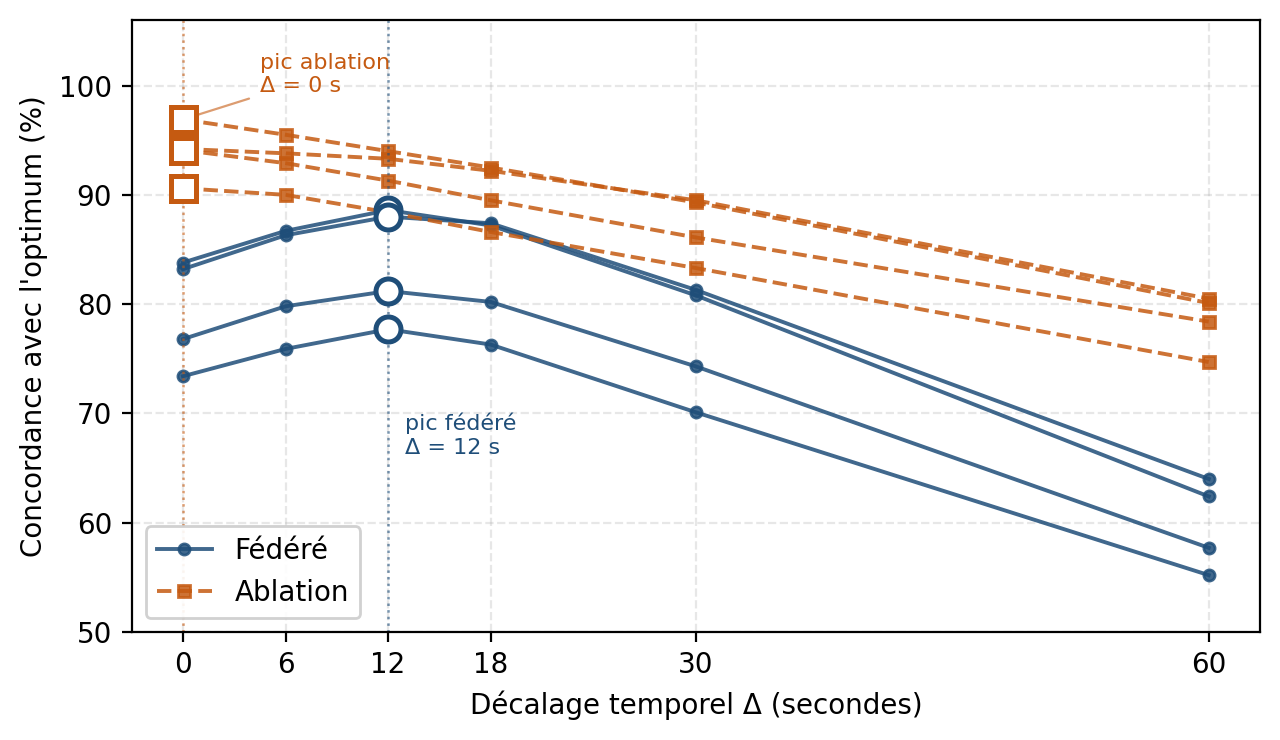
\includegraphics[width=0.95\textwidth]{images/fig_concordance.png}
    \caption{Concordance avec l'optimum selon le décalage temporel $\Delta$. Les cercles évidés marquent le maximum de chaque exécution.}
    \label{fig:concordance}
\end{figure}

Le résultat se reproduit sans exception sur les huit exécutions indépendantes, comme le montre la figure~\ref{fig:concordance}. Les quatre exécutions fédérées atteignent toutes leur maximum de concordance à $\Delta = 12$~s, tandis que les quatre exécutions d'ablation l'atteignent toutes à $\Delta = 0$~s. Aucune exécution ne fait exception et, dans les huit cas, le taux de concordance décroît de manière régulière de part et d'autre du maximum. Cette reproductibilité indique que le phénomène observé ne semble pas dépendre d'une seule exécution ou d'une fenêtre de mesure particulière.

En configuration fédérée, la décision suit donc l'optimum avec un retard d'environ douze secondes, soit deux cycles complets. Le système ne sélectionne pas nécessairement une cible intrinsèquement inadéquate : il tend à sélectionner une cible qui correspond à l'optimum observé deux cycles plus tôt.

Rapporté à la dynamique du banc d'essai, ce retard reste modeste dans l'absolu. Le véhicule progresse à vingt-cinq millimètres par seconde ; en douze secondes, il parcourt donc trois centimètres, alors que le rayon de la zone dans laquelle le seuil de latence est respecté avoisine quinze centimètres. Traverser une telle zone de part en part demande ainsi de l'ordre de deux minutes et le retard de décision en représente environ un dixième. Le système ne se trompe donc pas de région : il présente plutôt un décalage de phase à l'intérieur d'un mouvement qu'il suit correctement par ailleurs.

Cette modestie apparente ne doit toutefois pas conduire à en minimiser l'effet. Douze secondes suffisent pour que le véhicule franchisse une frontière de zone, et c'est précisément aux abords de ces frontières que la décision devient déterminante. Au milieu d'une zone, plusieurs cibles peuvent en effet présenter un comportement comparable. Le retard ne dégrade donc pas nécessairement la qualité de service de manière uniforme : son effet se concentre principalement lors des transitions, lorsque le placement doit s'adapter à l'évolution de la position du véhicule.

L'absence apparente de retard en ablation demande une lecture prudente. Il serait tentant d'en conclure que le mode mono-fournisseur décide plus rapidement. Une autre interprétation, cohérente avec la configuration expérimentale, est que les quatre cibles, toutes situées chez le même fournisseur, offrent moins d'occasions de changement de VM optimale. Un retard de deux cycles peut alors rester difficile à observer, puisque l'optimum n'a, dans de nombreux cas, pas changé pendant cet intervalle. Les résultats ne permettent donc pas d'affirmer que le retard est absent en configuration d'ablation ; ils montrent qu'il n'est pas mis en évidence par cette mesure. Le doublement du nombre de cibles ne crée donc pas nécessairement le retard : il peut également le rendre plus observable.

Ce retard est associé à un coût mesurable. Le classement des violations selon qu'une VM conforme existait ou non au même instant permet de le quantifier :

\begin{table}[H]
    \centering
    \caption{Nature des violations selon la configuration (moyenne sur quatre exécutions par condition)}
    \label{tab:violations-evitables}
    \begin{tabular}{lcc}
        \toprule
        \textbf{Nature des violations} & \textbf{Fédéré} & \textbf{Ablation} \\
        \midrule
        Violations inévitables (aucune VM conforme) & 7,6~\% & 53,2~\% \\
        Violations évitables (une VM conforme existait) & 16,3~\% & 1,7~\% \\
        \bottomrule
    \end{tabular}
\end{table}

En ablation, la majorité des violations est inévitable : aucune des quatre cibles n'était conforme à l'instant considéré et aucun choix parmi les cibles disponibles n'aurait pu éviter la violation. En configuration fédérée, la situation est différente : la proportion de violations inévitables tombe à 7,6~\%, tandis que 16,3~\% du temps correspond à des situations dans lesquelles une cible conforme existait sans avoir été retenue. Ces violations évitables sont compatibles avec l'existence du retard mis en évidence par l'analyse précédente : une cible conforme était disponible, mais elle n'était pas encore sélectionnée au moment considéré.

\textbf{Une cause candidate a été identifiée, puis testée.} L'agrégation des prédictions sur l'horizon repose sur une moyenne pondérée dont les poids décroissent linéairement. Le premier pas prédit reçoit ainsi un poids de 7 sur un total de 28, soit 25~\% de l'ensemble, tandis que le septième n'en reçoit que 3,6~\%. La valeur agrégée est donc davantage influencée par les prédictions les plus proches, ce qui pourrait contribuer à un comportement davantage réactif qu'anticipatif. Un profil de pondération recentré sur les deuxième et troisième pas, correspondant à l'horizon utile de deux cycles, constituait donc une piste de correction cohérente avec le retard observé.

Cette hypothèse n'ayant pas pu être vérifiée pendant la campagne — le principe retenu interdisait de modifier un paramètre entre deux exécutions — elle a fait l'objet d'une exécution supplémentaire menée ultérieurement, sur la même trajectoire et dans la même configuration fédérée. Le profil de pondération y était remplacé par $[3,5,5,4,3,2,1]$, plaçant le maximum sur les deuxième et troisième pas. Le critère de réussite avait été fixé avant l'exécution : le maximum de concordance devait se déplacer vers $\Delta = 6$~s ou $\Delta = 0$~s.

\begin{table}[H]
    \centering
    \caption{Effet du profil de pondération recentré (exécution supplémentaire)}
    \label{tab:run9-horizon}
    \begin{tabular}{lrr}
        \toprule
        \textbf{Indicateur} & \textbf{Campagne (4 exécutions)} & \textbf{Profil recentré} \\
        \midrule
        Maximum de concordance & $\Delta = 12$~s & $\Delta = 12$~s \\
        Concordance à $\Delta = 6$~s & 82,2~\% & 79,3~\% \\
        Concordance à $\Delta = 12$~s & 83,9~\% & 79,8~\% \\
        \addlinespace
        Taux de violation & 23,8~\% (19,9 -- 29,3) & 26,5~\% \\
        Violations évitables & 16,3~\% (12,2 -- 21,8) & 19,2~\% \\
        Migrations / 100 cycles & 7,0 (6,5 -- 7,3) & 6,1 \\
        \bottomrule
    \end{tabular}
\end{table}

\textbf{Le critère n'est pas atteint : le maximum reste à douze secondes.} L'hypothèse selon laquelle la pondération de l'horizon serait la cause du retard n'est donc pas confirmée. Sur les autres indicateurs, l'exécution ne se distingue pas des quatre exécutions fédérées de la campagne : taux de violation et violations évitables restent dans leur étendue respective, et la fréquence des migrations demeure comparable, ce qui écarte au passage un effet oscillatoire du nouveau profil.

Un élément mérite néanmoins d'être relevé sans être surinterprété : l'écart de concordance entre $\Delta = 6$~s et $\Delta = 12$~s, compris entre 1,4 et 1,9 point sur les quatre exécutions de la campagne, tombe à 0,5 point ici. Le maximum s'aplatit sans se déplacer. Cette observation, issue d'une exécution unique et menée avec des modèles de prédiction réentraînés entre-temps, ne permet pas de conclure à un effet partiel de la modification.

\textbf{Le retard de suivi reste donc une limite mesurée dont la cause n'est pas établie.} La formulation retenue ici est délibérément prudente : l'hypothèse la plus immédiate a été testée dans les conditions de la campagne et n'a pas été confirmée, ce qui exclut une explication et en laisse d'autres ouvertes — durée du cycle, délai de propagation des migrations, ou combinaison de plusieurs facteurs. Ce point est repris parmi les pistes d'amélioration en section~\ref{sec:limites-ameliorations}.

\subsection{Stabilité des décisions}
\label{sec:stabilite-decisions}

Une décision juste, mais prise trop fréquemment, peut devenir coûteuse. Chaque migration entraîne le déplacement effectif d'un pod entre deux machines, avec l'interruption de service que cela implique. Un orchestrateur qui basculerait à chaque cycle vers la cible marginalement la mieux classée serait difficilement exploitable, même si chacun de ses choix était localement justifié. La stabilité n'est donc pas une qualité accessoire du système : elle constitue une condition de son utilisabilité.

Trois garde-fous contribuent à cette stabilité. Une marge d'hystérésis exige qu'une cible candidate dépasse la cible active de plus de cinq pour cent en termes de score multicritère avant qu'une migration ne soit envisagée ; en deçà de ce seuil, le système conserve son placement. Un délai de garde interdit toute nouvelle migration pendant les secondes qui suivent la précédente. Enfin, en configuration fédérée, l'arbitre applique une bande morte absolue sur l'écart entre les offres, afin d'éviter un changement de fournisseur lorsqu'un concurrent n'est que marginalement meilleur.

\textbf{Méthode.} Le nombre de migrations effectivement déclenchées a été relevé dans les journaux de décision de chaque exécution. Les durées d'exécution différant sensiblement, les valeurs brutes ne sont pas directement comparables ; elles sont donc rapportées sous forme d'un taux pour cent cycles d'orchestration. En configuration fédérée, le service peut être déplacé par l'un ou l'autre des deux orchestrateurs. Les migrations des deux fournisseurs sont donc cumulées, tandis que le nombre de cycles du premier sert de référence temporelle, les deux orchestrateurs opérant à la même cadence.

\begin{table}[H]
    \centering
    \caption{Fréquence des migrations par condition}
    \label{tab:frequence-migrations}
    \begin{tabular}{llrrr}
        \toprule
        \textbf{Exécution} & \textbf{Condition} & \textbf{Cycles} & \textbf{Migrations} & \textbf{Taux (/100 cycles)} \\
        \midrule
        UC1  & fédéré   & 462 & 30 & 6,5 \\
        FED1 & fédéré   & 475 & 34 & 7,2 \\
        FED2 & fédéré   & 491 & 34 & 6,9 \\
        FED3 & fédéré   & 931 & 68 & 7,3 \\
        \addlinespace
        UC2  & ablation & 406 & 16 & 3,9 \\
        ABL1 & ablation & 402 & 29 & 7,2 \\
        ABL2 & ablation & 566 & 72 & 12,7 \\
        ABL3 & ablation & 630 & 55 & 8,7 \\
        \midrule
        \multicolumn{2}{l}{\textbf{Fédéré} — taux moyen}   & \multicolumn{2}{r}{\textbf{7,0}} & étendue 6,5 -- 7,3 \\
        \multicolumn{2}{l}{\textbf{Ablation} — taux moyen} & \multicolumn{2}{r}{\textbf{8,2}} & étendue 3,9 -- 12,7 \\
        \bottomrule
    \end{tabular}
\end{table}

Aucune configuration ne présente, au regard de ces mesures, de comportement oscillatoire manifeste. Un taux de sept migrations pour cent cycles correspond à environ une migration toutes les quatorze cycles, soit près d'une minute et demie. Cette durée est à rapprocher des deux minutes nécessaires au véhicule pour traverser une zone de conformité. Le rythme des migrations est donc compatible avec la dynamique du déplacement plutôt qu'avec une succession rapide de basculements entre les cibles. Les garde-fous semblent ainsi limiter les migrations excessivement fréquentes dans les deux configurations.

Le premier résultat est contre-intuitif : doubler le nombre de cibles n'augmente pas la fréquence des migrations. On pourrait s'attendre à l'inverse, dans la mesure où un ensemble de choix plus large offre davantage d'occasions de basculer. Le taux moyen est pourtant légèrement inférieur en configuration fédérée qu'en ablation. Une explication possible tient davantage à la qualité et à la disponibilité temporelle des cibles qu'à leur seul nombre : lorsqu'une cible conforme est disponible, elle peut le rester plusieurs cycles, ce qui limite les changements successifs.

Le second résultat concerne la régularité observée entre les exécutions. Les quatre exécutions fédérées s'inscrivent dans un intervalle de 6,5 à 7,3 migrations pour cent cycles, soit une étendue de 0,8 point. Les quatre exécutions d'ablation s'échelonnent de 3,9 à 12,7, soit une étendue de 8,8 points, plus de dix fois supérieure. Alors même que la trajectoire du véhicule est identique d'une exécution à l'autre, le taux de migration varie davantage entre les exécutions en configuration d'ablation que dans la configuration fédérée.

Cette dispersion en ablation n'a pas reçu d'explication établie. L'hypothèse la plus immédiate — selon laquelle un nombre plus faible de cibles conformes conduirait le système à rechercher davantage d'alternatives — ne suffit pas à expliquer les résultats observés. En effet, la proportion de violations inévitables, rapportée en section~\ref{sec:retard-suivi}, est pratiquement identique entre l'exécution présentant le taux de migration le plus faible et celle présentant le taux le plus élevé : 52,9~\% contre 53,0~\%, alors que leurs taux de migration diffèrent d'un facteur supérieur à trois. La cause de cette variabilité reste donc à caractériser et est rapportée comme telle, sans lui attribuer d'explication non vérifiée.

Sous cette réserve, la régularité observée dans la configuration fédérée constitue un résultat favorable : sur les quatre exécutions considérées, la fréquence des migrations varie moins que dans la configuration d'ablation. Ces résultats suggèrent que, dans les conditions évaluées, la décision issue de la négociation entre fournisseurs est moins variable d'une exécution à l'autre que celle prise par un fournisseur isolé.

\newpage
\section{Résultats : fédération}
\label{sec:resultats-federation}

Les sections précédentes ont évalué les composants du système et le comportement d'un fournisseur isolé. Celle-ci répond à la question qui a motivé l'ensemble du travail : la coopération entre fournisseurs indépendants améliore-t-elle effectivement le respect des objectifs de qualité de service ? Trois aspects sont examinés : la réduction du taux de violation (section~\ref{sec:federation-reduit-violation}), la part du gain théoriquement atteignable effectivement capturée (section~\ref{sec:gain-capture}), et le comportement du système lors du passage de relais entre fournisseurs (section~\ref{sec:passage-relais}).

\subsection{La fédération réduit le taux de violation}
\label{sec:federation-reduit-violation}

C'est le résultat central de ce travail. La problématique posée au chapitre~1 supposait qu'un fournisseur seul ne peut pas toujours honorer une intention, et que la coopération avec ses pairs devrait permettre d'y parvenir. Cette hypothèse est ici confrontée à la mesure, sur huit exécutions indépendantes.

\begin{table}[H]
    \centering
    \caption{Taux de violation par exécution}
    \label{tab:taux-violation}
    \begin{tabular}{llrrr}
        \toprule
        \textbf{Exécution} & \textbf{Condition} & \textbf{Durée} & \textbf{Échantillons en violation} & \textbf{Taux} \\
        \midrule
        UC1  & fédéré   & 52,8~min  & 315 / 1\,586  & 19,9~\% \\
        FED1 & fédéré   & 55,7~min  & 422 / 1\,627  & 25,9~\% \\
        FED2 & fédéré   & 57,0~min  & 502 / 1\,712  & 29,3~\% \\
        FED3 & fédéré   & 108,4~min & 656 / 3\,252  & 20,2~\% \\
        \addlinespace
        UC2  & ablation & 40,5~min  & 652 / 1\,215  & 53,7~\% \\
        ABL1 & ablation & 44,3~min  & 701 / 1\,331  & 52,7~\% \\
        ABL2 & ablation & 57,4~min  & 973 / 1\,720  & 56,6~\% \\
        ABL3 & ablation & 63,1~min  & 1\,067 / 1\,894 & 56,3~\% \\
        \midrule
        \multicolumn{2}{l}{\textbf{Fédéré} — moyenne}   & \multicolumn{2}{r}{\textbf{23,8~\%}} & $\sigma$ = 4,6~pt \\
        \multicolumn{2}{l}{\textbf{Ablation} — moyenne} & \multicolumn{2}{r}{\textbf{54,8~\%}} & $\sigma$ = 1,9~pt \\
        \bottomrule
    \end{tabular}
\end{table}

L'écart est de \textbf{31,0 points} en faveur de la configuration fédérée, soit une réduction de 57~\% du temps passé en violation.

\begin{figure}[H]
    \centering
    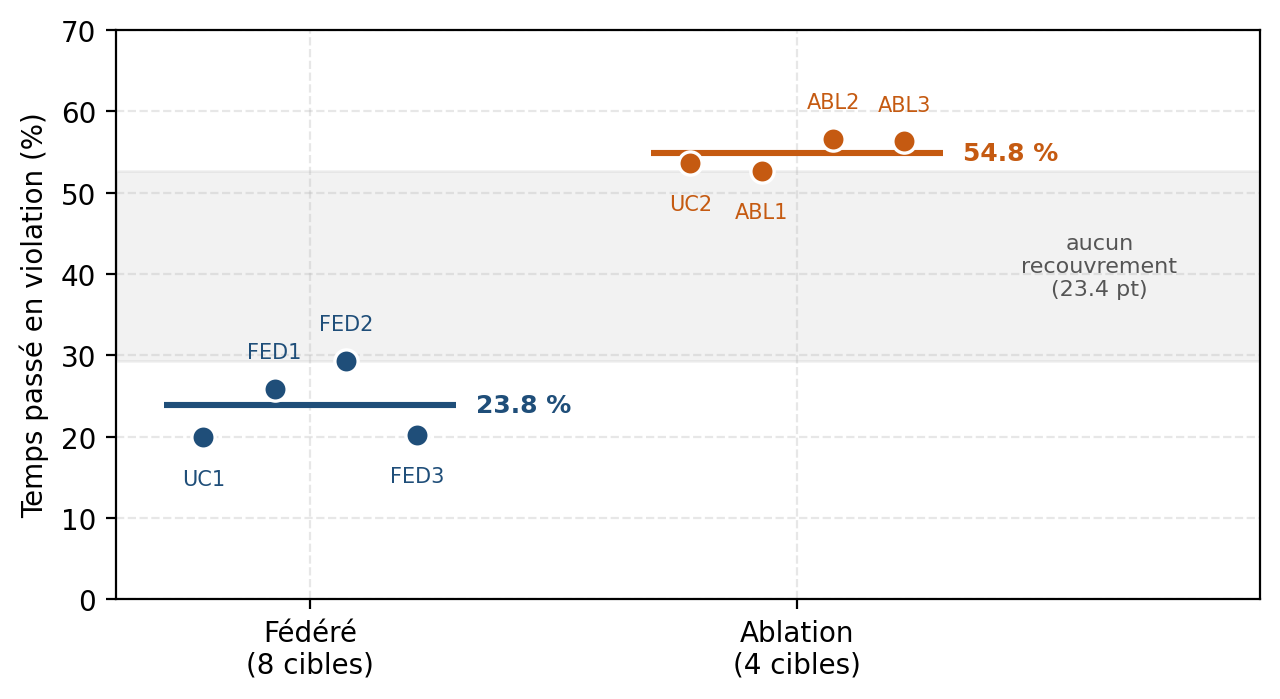
\includegraphics[width=0.92\textwidth]{images/fig_violation.png}
    \caption{Taux de violation des huit exécutions. Les traits horizontaux indiquent la moyenne de chaque condition ; la bande grisée matérialise l'intervalle où aucune exécution ne tombe.}
    \label{fig:violation}
\end{figure}

\textbf{Les deux groupes ne se recouvrent pas.} La pire exécution fédérée (29,3~\%) reste inférieure de plus de vingt-trois points à la meilleure exécution d'ablation (52,7~\%). Cette séparation stricte est une propriété forte : elle signifie que le classement des huit exécutions place les quatre exécutions fédérées avant les quatre exécutions d'ablation, sans exception.

Le test exact de Mann-Whitney, justifié en section~\ref{sec:protocole-metriques}, confirme cette lecture : $U = 16{,}0$ et $p = 0{,}0286$. La statistique $U$ atteint sa valeur maximale, ce qui correspond précisément à l'absence de recouvrement entre les deux groupes. La valeur de $p$ obtenue est la plus petite atteignable avec quatre observations par condition : le résultat est significatif au seuil de 5~\%, et il l'est autant que la taille de l'échantillon le permet. Aucune configuration de ces huit mesures ne pourrait produire une p-valeur inférieure.

\textbf{Ce que ce résultat établit, et ce qu'il n'établit pas.} Il établit que, sur ce banc d'essai et pour cette trajectoire, l'accès aux cibles d'un second fournisseur réduit très significativement le temps passé en violation. La seule différence entre les deux conditions étant l'activation de la fédération — même trajectoire, même seuil, même code — l'écart lui est attribuable.

Il n'établit pas que le gain provient de la qualité de la décision. La section~\ref{sec:gain-capture} montre au contraire qu'il provient d'abord de l'élargissement de la couverture physique : avec quatre cibles seulement, aucune n'est conforme plus de la moitié du temps, et aucun algorithme, si bon soit-il, ne pourrait éviter ces violations.

\textbf{Trois réserves accompagnent ce résultat.}

D'abord, quatre exécutions par condition suffisent à établir une différence, non à la caractériser. Elles bornent une moyenne et une dispersion, mais ne disent rien de la forme de la distribution sous-jacente et n'autorisent aucun diagnostic de valeur aberrante. Les exécutions fédérées diffèrent entre elles de 9,4 points, et cette dispersion n'a pas reçu d'explication établie.

Ensuite, les deux chemins de décision ne partagent pas exactement la même politique de dernier recours. Lorsque aucune cible ne satisfait le contrat, le chemin fédéré déclare l'intention infaisable plutôt que de retenir une offre non conforme — un fournisseur n'exporte jamais vers un pair un placement qu'il sait en infraction — tandis que le chemin mono-fournisseur retient la moins mauvaise cible disponible. Cette asymétrie est délibérée, mais elle signifie que les deux conditions ne diffèrent pas uniquement par le nombre de cibles. Son effet reste toutefois borné : elle ne s'applique que lorsque aucune cible conforme n'existe, et l'écart mesuré est d'un ordre de grandeur supérieur à toute contribution plausible de ce mécanisme.

Enfin, une neuvième exécution fédérée a été menée après la campagne, avec un profil de pondération modifié (section~\ref{sec:retard-suivi}). Exécutée avec un code différent des huit autres, elle n'entre ni dans les moyennes rapportées ici ni dans le test statistique.

\subsection{Part du gain atteignable capturée}
\label{sec:gain-capture}

Le résultat précédent établit un écart entre les deux conditions ; il ne dit rien de la part de cet écart imputable à la qualité des décisions plutôt qu'à l'étendue du choix disponible. Deux bornes permettent de situer chaque système entre ce qu'aucun algorithme ne pourrait éviter et ce qu'un placement figé, sans aucune décision, obtiendrait déjà.

\textbf{Méthode.} Pour chaque instant, la borne oracle retient la VM offrant la plus faible latence à cet instant précis, ce qu'aucun système réel ne peut faire puisqu'elle suppose une connaissance parfaite et instantanée de l'état de toutes les cibles. La borne du meilleur placement statique retient, sur toute l'exécution, la VM unique qui minimise le taux de violation si le service y restait sans jamais migrer — c'est le comportement d'un ordonnanceur Kubernetes ordinaire, qui place une fois et ne réévalue pas.

\begin{table}[H]
    \centering
    \caption{Bornes de comparaison — configuration fédérée}
    \label{tab:bornes-federe}
    \begin{tabular}{lrrrr}
        \toprule
        \textbf{Exécution} & \textbf{Oracle} & \textbf{Système} & \textbf{Meilleur statique} & \textbf{Gain capturé} \\
        \midrule
        UC1  &  7,6~\% & 19,9~\% & 81,8~\% & 83~\% \\
        FED1 &  7,4~\% & 25,9~\% & 80,7~\% & 75~\% \\
        FED2 &  7,5~\% & 29,3~\% & 82,2~\% & 71~\% \\
        FED3 &  7,6~\% & 20,2~\% & 82,7~\% & 83~\% \\
        \midrule
        \textbf{Moyenne} & \textbf{7,5~\%} & \textbf{23,8~\%} & \textbf{81,9~\%} & \textbf{78~\%} \\
        \bottomrule
    \end{tabular}
\end{table}

\begin{table}[H]
    \centering
    \caption{Bornes de comparaison — configuration d'ablation}
    \label{tab:bornes-ablation}
    \begin{tabular}{lrrrr}
        \toprule
        \textbf{Exécution} & \textbf{Oracle} & \textbf{Système} & \textbf{Meilleur statique} & \textbf{Gain capturé} \\
        \midrule
        UC2  & 52,9~\% & 53,7~\% & 82,3~\% & 97~\% \\
        ABL1 & 51,8~\% & 52,7~\% & 83,0~\% & 97~\% \\
        ABL2 & 53,0~\% & 56,6~\% & 83,4~\% & 88~\% \\
        ABL3 & 54,9~\% & 56,3~\% & 84,2~\% & 95~\% \\
        \midrule
        \textbf{Moyenne} & \textbf{53,1~\%} & \textbf{54,8~\%} & \textbf{83,2~\%} & \textbf{94~\%} \\
        \bottomrule
    \end{tabular}
\end{table}

\begin{figure}[H]
    \centering
    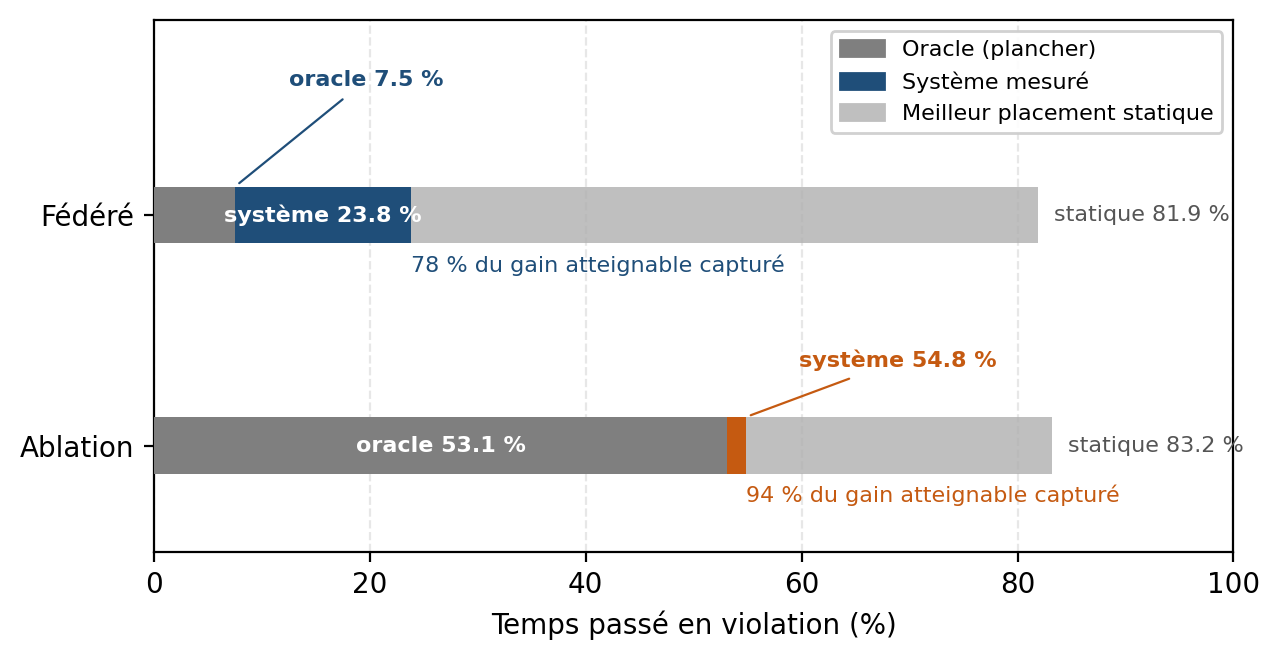
\includegraphics[width=0.95\textwidth]{images/fig_bornes.png}
    \caption{Position du système entre ses deux bornes, par condition. La fédération abaisse l'oracle de 53,1~\% à 7,5~\% : c'est l'atteignable lui-même qui se déplace.}
    \label{fig:bornes}
\end{figure}

\textbf{L'ablation capture presque tout son gain atteignable ; le fédéré, non.} En configuration d'ablation, le système mesuré s'écarte de son propre oracle de 0,8 à 3,6 points seulement selon l'exécution — il capture en moyenne 94~\% du gain théoriquement atteignable compte tenu des quatre cibles disponibles. En configuration fédérée, cet écart monte à 12,3--21,8 points, pour une capture moyenne de 78~\%.

Cette asymétrie répond directement à la question laissée ouverte en section~\ref{sec:federation-reduit-violation} : le gain observé ne provient pas d'une décision meilleure en fédéré qu'en ablation — c'est l'inverse qui est mesuré. Il provient de l'élargissement du choix disponible : doubler le nombre de cibles déplace l'oracle de 53,1~\% à 7,5~\%, soit 45,6 points gagnés par la seule extension de la couverture, avant même toute décision.

\textbf{Ce que cet écart de capture révèle.} Que le fédéré capture une part moindre de son gain atteignable n'indique pas un défaut de conception spécifique à la fédération : il est cohérent avec le retard de suivi de douze secondes mesuré en section~\ref{sec:retard-suivi}, qui n'affecte que la configuration fédérée. FED1 et FED2, les deux exécutions où cet écart est le plus marqué (75~\% et 71~\%), sont aussi celles où la proportion de violations évitables est la plus élevée (section~\ref{sec:retard-suivi}) — cohérence supplémentaire entre deux mesures obtenues par des méthodes indépendantes.

\subsection{Comportement lors du passage de relais}
\label{sec:passage-relais}

Le mécanisme de fédération n'est pertinent que si le passage du service d'un fournisseur à l'autre se déroule sans ambiguïté ni retard excessif. Cette section illustre ce mécanisme sur un exemple réel, tiré des journaux de l'exécution FED3.

\textbf{Le déclencheur.} Au cycle 3, l'arbitre de provider-2 propose \texttt{edge2} avec un Gap Grade de $-0{,}7151$, contre $-0{,}0239$ pour le tenant en place chez provider-1 — un écart qui dépasse la bande morte de $0{,}05$ retenue pour éviter les changements de fournisseur marginaux. La migration est déclenchée.

\begin{table}[H]
    \centering
    \caption{Séquence d'un passage de relais réel (FED3, cycle 3)}
    \label{tab:passage-relais}
    \begin{tabular}{lp{7.5cm}}
        \toprule
        \textbf{Horodatage} & \textbf{Événement} \\
        \midrule
        12:20:52 & Décision \texttt{migrate edge1 → edge2} enregistrée côté provider-1 \\
        12:20:53 & Migration \texttt{kubectl} exécutée (190~ms) ; \texttt{/award} envoyé à provider-2 \\
        12:20:54 & \texttt{/award} livré ; provider-1 passe en \textbf{STANDBY} ; provider-2 passe en \textbf{ACTIF} \\
        12:20:56 & Une synchronisation \texttt{kubectl} périmée arrive côté provider-2 ; ignorée grâce à la fenêtre de grâce, le rôle ACTIF est conservé \\
        \bottomrule
    \end{tabular}
\end{table}

\textbf{Le rôle de la fenêtre de grâce.} Deux secondes après avoir reçu l'attribution, provider-2 reçoit une resynchronisation \texttt{kubectl} qui reflète encore l'état antérieur à la migration. Sans protection, cette resynchronisation aurait pu ramener provider-2 en STANDBY alors qu'il vient tout juste de prendre le service — un split-brain de courte durée, où aucun des deux fournisseurs ne se considérerait actif. La fenêtre de grâce qui suit chaque \texttt{award} neutralise précisément ce cas : le journal l'indique explicitement (\og~synchronisation kubectl périmée ignorée, fenêtre de grâce award, rôle conservé : ACTIF~\fg{}).

\textbf{Durée totale.} Depuis la décision jusqu'à la confirmation du nouveau rôle, la séquence complète prend environ 4,3 secondes sur cet exemple, migration \texttt{kubectl} et transmission de l'attribution comprises — un ordre de grandeur inférieur au cycle d'orchestration de six secondes, ce qui évite qu'un passage de relais empiète sur le suivant.

\newpage
\section{Synthèse et limites}
\label{sec:synthese-limites}

\subsection{Bilan par rapport à la problématique}
\label{sec:bilan-problematique}

La problématique posée au chapitre~1 interrogeait la capacité d'un fournisseur isolé à honorer une intention de qualité de service, et proposait la coopération entre fournisseurs comme réponse. Les résultats de ce chapitre y répondent, avec les nuances que la mesure impose.

\textbf{La chaîne fonctionne de bout en bout.} Une intention en langage naturel est traduite en contrat SLO pondéré (section~\ref{sec:fidelite-interpretation}), y compris sur des formulations non conçues pour le système ; les deux demandes hors périmètre sont déclinées plutôt que mal interprétées (section~\ref{sec:comportement-repli}). Le contrat pilote ensuite une décision locale informée par la prédiction (section~\ref{sec:qualite-prediction}) et, potentiellement, par une métrique secondaire découverte (section~\ref{sec:validation-mi}).

\textbf{La fédération répond positivement à la problématique.} L'accès aux cibles d'un second fournisseur réduit le taux de violation de 54,8~\% à 23,8~\% (section~\ref{sec:federation-reduit-violation}), un écart significatif au seuil de 5~\%. Ce gain provient majoritairement de l'élargissement du choix disponible plutôt que d'une décision plus fine : le système capture 94~\% de son gain atteignable en ablation contre 78~\% en fédéré (section~\ref{sec:gain-capture}) — la fédération élargit ce qui est atteignable, plus qu'elle n'améliore la façon de l'atteindre.

\textbf{Cette réponse reste bornée.} Un retard de suivi de douze secondes (section~\ref{sec:retard-suivi}) et une dispersion inter-exécutions non expliquée (section~\ref{sec:limites-ameliorations}) limitent la part du gain effectivement capturée. La coopération entre fournisseurs n'élimine donc pas toute violation ; elle déplace substantiellement la limite de ce qui est atteignable, et le système en capture une majorité, sans encore l'épuiser.

\subsection{Limites et pistes d'amélioration}
\label{sec:limites-ameliorations}

Cette section rassemble les limites identifiées au fil du chapitre, avec pour chacune ce qui a déjà été testé, ce qui reste ouvert, et pourquoi certaines ne sont pas traitées comme des défauts à corriger.

\textbf{Le retard de suivi.} L'hypothèse des poids d'horizon (section~\ref{sec:retard-suivi}) a été testée et n'a pas été confirmée. Deux pistes recensées avant la campagne restent, elles, non testées : réduire la période du cycle (6~s~$\rightarrow$~3~s), qui diviserait mécaniquement le retard mais recouple l'ensemble des grandeurs temporelles du banc (horizon de prédiction, fenêtre d'historique, cooldown) et exige une étude de dimensionnement préalable — cette modification est reportée à une itération ultérieure, une fois cette étude menée ; et réduire le délai de garde entre deux migrations, plus simple mais avec un risque d'oscillation à surveiller. Une piste supplémentaire a été identifiée après la campagne : le temps de négociation entre fournisseurs, mesuré entre 2,6 et 3,2 secondes lorsqu'elle a lieu, pousse certains cycles au-delà du budget nominal de 6~s — cohérent avec le retard mesuré, sans être confirmé comme cause unique. L'examen du code a révélé qu'une connexion réseau neuve était ouverte à chaque négociation, sans réutilisation. Le correctif correspondant, mesuré sur trente négociations consécutives dans les conditions du banc, ramène le temps de négociation de 2\,392~ms à 881~ms en médiane, soit une réduction de 63~\%. Cette accélération est établie ; son effet sur le retard de suivi ne l'est pas, faute d'un nombre d'exécutions suffisant pour le distinguer de la variabilité déjà observée entre exécutions.

\textbf{Le plancher du Gap Grade.} La borne \texttt{DELTA\_FLOOR} limite l'écart normalisé à $-1$ au minimum. Sans elle, un excédent extrême sur un critère secondaire peut dominer la somme pondérée et l'emporter sur un critère primaire pourtant plus fragile — l'exemple illustratif suivant, construit pour deux SLO pondérés (latence $< 65$~ms, poids $0{,}6$ ; CPU disponible $\geq 2{,}5$~cœurs, poids $0{,}4$), le montre.

\begin{table}[H]
    \centering
    \caption{Exemple illustratif — deux VM conformes}
    \label{tab:floor-exemple-entree}
    \begin{tabular}{lccc}
        \toprule
        \textbf{VM} & \textbf{Latence} & \textbf{CPU disponible} & \textbf{Conforme} \\
        \midrule
        cloud1 & 60~ms & 12,8~cœurs & oui \\
        edge2  & 32~ms &  3,2~cœurs & oui \\
        \bottomrule
    \end{tabular}
\end{table}

\begin{table}[H]
    \centering
    \caption{Écarts normalisés, avant et après plancher}
    \label{tab:floor-exemple-ecarts}
    \begin{tabular}{lrrr}
        \toprule
        \textbf{VM} & $\delta_{\text{latence}}$ & $\delta_{\text{CPU}}$ (brut) & $\delta_{\text{CPU}}$ (planché) \\
        \midrule
        cloud1 & $-0{,}077$ & $-4{,}120$ & $-1{,}000$ \\
        edge2  & $-0{,}508$ & $-0{,}280$ & $-0{,}280$ \\
        \bottomrule
    \end{tabular}
\end{table}

\begin{table}[H]
    \centering
    \caption{Gap Grade résultant, avant et après plancher}
    \label{tab:floor-exemple-resultat}
    \begin{tabular}{lrr}
        \toprule
        \textbf{VM} & \textbf{Sans plancher} & \textbf{Avec plancher} \\
        \midrule
        cloud1 & $-0{,}196$ \textbf{(gagne)} & $-0{,}083$ \\
        edge2  & $-0{,}140$ & $-0{,}140$ \textbf{(gagne)} \\
        \bottomrule
    \end{tabular}
\end{table}

Sans plancher, cloud1 l'emporte : son excédent de CPU écrase la somme pondérée malgré une marge de latence de seulement 5~ms sur un seuil de 65~ms. Avec plancher, edge2 l'emporte — la VM dont la marge est la plus confortable sur le critère le plus pondéré. Le plancher reste une limite au sens strict — il efface une information réelle sur un critère pris isolément — mais il constitue une correction nécessaire au comportement global de l'arbitrage, pas un défaut à corriger.

\textbf{Dispersion inter-exécutions.} Les quatre exécutions fédérées diffèrent entre elles de 9,4 points de taux de violation (section~\ref{sec:federation-reduit-violation}), sans explication établie.

\textbf{Vérification FED1/ABL2.} Deux exécutions de la campagne (FED1, ABL2) avaient fait l'objet d'un doute sur un réentraînement involontaire du modèle ML en cours de run. Vérification faite sur l'erreur de prédiction de latence, tranche par tranche : aucune cassure détectée après la période d'échauffement initiale déjà documentée — l'erreur reste stable et basse jusqu'à la fin des deux exécutions. Cette vérification ne couvre que la prédiction de latence ; elle ne permet pas d'exclure un effet sur les décisions elles-mêmes.

\textbf{Fédération sur deux machines physiques distinctes.} Cette configuration reste bloquée par une limitation de \texttt{launch\_provider.py}, non résolue au moment de la rédaction.

\newpage
\section{Conclusion}
\label{sec:tests-conclusion}

Ce chapitre a soumis xQoS à l'épreuve de la mesure, sur l'infrastructure réelle du LAAS-CNRS plutôt qu'en simulation. Deux échelles distinctes ont structuré cette évaluation : la décision locale, prise par un seul fournisseur à partir de ses propres cibles, et la décision fédérée, qui ouvre ce choix à un pair par négociation.

À l'échelle locale, la traduction d'intention, la prédiction et la découverte de métriques secondaires fonctionnent de bout en bout, avec des limites précisément mesurées plutôt que supposées : une découverte MI d'abord invalidée par le banc d'essai puis validée après correction (section~\ref{sec:validation-mi}), un retard de suivi de deux cycles dont une cause candidate a été testée et écartée (section~\ref{sec:retard-suivi}), un plancher de score dont l'effet a été démontré nécessaire plutôt que simplement toléré (section~\ref{sec:limites-ameliorations}).

À l'échelle fédérée, le résultat central tient en une phrase : ouvrir la décision à un second fournisseur réduit le temps passé en violation de plus de moitié, un écart significatif malgré la petite taille de l'échantillon. Ce gain s'explique d'abord par la couverture physique élargie, et seulement ensuite par la qualité de la décision (section~\ref{sec:gain-capture}) — une distinction que seule la mesure, et non l'intuition, pouvait établir.

Ces résultats répondent à la problématique du chapitre~1 sans la clore (section~\ref{sec:bilan-problematique}) : ils établissent qu'une fédération d'intent-based orchestrators réduit mesurablement les violations de qualité de service sur ce banc d'essai, et documentent avec la même rigueur ce qui reste à améliorer.
